\hyphenation{
Barrow
Binet
Cavalieri
Cotes
Chebyshev
Cholesky
Cramer
Gauss
Faber
Hausdorff
Householder
Lagrange
Laplace
Lebesque
Newton
Rolle
Runghe
Simpson
Sturm
tras-for-ma-zio-ne
Torricelli
}

\chapter{Integrazione Numerica.}
\textbf{Problema:}\\ \emph{calcolo numerico} dell'integrale definito di una
funzione $f \colon [a,b] \to \rr$, integrabile in $[a,b]$,  cioé $\int_a^b
f(x)dx$ mediante una formula del tipo:
\[\sum_{i=0}^n\omega_if(x_i) = \omega_0f(x_0)+ \omega_1f(x_1)+ \cdots 
+ \omega_nf(x_n),\]
dove $x_i \in [a,b], \ i = 0, \ldots, n$, sono detti \emph{nodi} e sono 
distinti, $\omega_i, \ i=0, \ldots, n$ sono detti \emph{pesi}.
\begin{flushleft}
\textbf{Analisi dell'errore:}
\[R_n(f) := \int_a^bf(x)dx - \sum_{i=0}^n\omega_if(x_i).\]
Possiamo calcolare $R_n(f)$ esattamente solo quando abbiamo $\int_a^bf(x)dx$,
quando non è possibile ricavare esattamente il valore dell'integrale è
possibile usare le formule di quadratura.
\end{flushleft}

\section{Formule (di quadratura) interpolatorie.}
Fissato $n \in \nn$ si scelgono $n+1$ nodi $\{x_i\}_{i=0}^n$ in $[a,b]$, con
$x_i \neq x_j$ per $i \neq j$; quindi si approssima $f(x)$ con il suo 
polinomio interpolatore $p_n(x)$ nei nodi fissati.
I punti base del polinomio sono: $x_0, \ldots, x_n$, in cui si calcolano i
valori della funzione: $f(x_0), \ldots, f(x_n)$.
\begin{osse}
$f(x)$ deve essere definita nei nodi di integrazione.
\end{osse}
Si ottiene allora:
\[\int_a^bf(x)dx = \int_a^bp_n(x)dx + \int_a^bE_n(x)dx.\]
\[\int_a^bf(x)dx = \sum_{i=0}^nf(x_i)\cdot \int_a^bL_i(x)dx + R_n(f).\]
$E_n(x)$ è l'errore di interpolazione, $L_i(x)$ sono i polinomi elementari di
Lagrange. Il \emph{resto} $R_n(f)$ è così definito:
\[R_n(f) = \int_a^bE_n(x)dx,\]
se $f \in \cc^{n+1}([a,b])$ si ha:
\[R_n(f) = \int_a^bw(x)\frac{f^{(n+1)}(\xi-x)}{(n+1)!}
dx.\]

Posto $\omega_i = \int_a^bL_i(x)dx, \ i = 0, \ldots, n$ si ottiene, 
trascurando il resto, la formula di quadratura:
\begin{equation}\label{eq14.1}
\int_a^bf(x)dx \simeq \sum_{i=0}^n\omega_if(x_i).
\end{equation} 

\begin{defi}La formula \ref{eq14.1}, in cui i pesi sono definiti da:
\[
\omega_i = \int_a^bL_i(x)dx, \quad i = 0, \ldots, n;
\]
viene detta formula di \emph{quadratura interpolatoria}.
\end{defi}

\begin{prop}
Una formula di quadratura interpolatoria integra esattamente almeno tutti
i polinomi di grado minore o uguale ad $n$.
\end{prop}
\begin{dimo}
Sia $p_n \in \PP_n$, allora:
\[R_n(f) = \int_a^bE_n(x)dx = \int_a^b\left(f(x)-p_n(x)\right)dx = 0.\]
Poiché $f(x) = p_n(x)$ per esistenza ed unicità del polinomio interpolante.
\end{dimo}

\begin{defi}
Una formula di quadratura si dice avere \emph{grado di precisione} $n$ se
integra esattamente tutti i polinomi di grado minore o uguale ad $n$ (resto
nullo) ed esiste $q \in \PP_{n+1}$ tale che $R_n(q) \neq 0$.
\end{defi}

\begin{osse}
Una formula di quadratura interpolatoria ha grado di precisione almeno $n$.
\end{osse}

\begin{teo}
Fissato $n \in \nn$, e fissati $n+1$ nodi distinti $\{x_i\}_{i=0}^n$ in $[a,b]$
esiste al più ($\exists!$) una formula di quadratura con grado di precisione
\emph{almeno} $n$, che quindi coincide con la formula di quadratura 
interpolatoria. 
\end{teo}

\begin{dimo}
Occorre imporre che $ \sum_{i=0}^n\omega_if(x_i)$ integri esattamente i 
polinomi di grado $\leq n$. Imponiamo quindi $n+1$ condizioni:
\[\left\{
\begin{array}{lr}
\sum_{i=0}^n\omega_i\cdot 1 = \int_a^b 1dx = b-a& x^{0} \\
\sum_{i=0}^n\omega_i\cdot x_i = \int_a^b xdx = \frac{b^2-a^2}{2}& x^{1} \\
\sum_{i=0}^n\omega_i\cdot x_i^2 = \int_a^b x^2dx = \frac{b^3-a^3}{3}& x^{2} \\
\vdots \\
\sum_{i=0}^n\omega_i\cdot x_i^n = \int_a^b x^ndx = 
\frac{b^{n+1}-a^{n+1}}{n+1}& x^{n}
\end{array}\right.
\]

\[\left\{
\begin{array}{l}
\omega_0 + \omega_1 + \cdots + \omega_n = b-a \\
\omega_0x + \omega_1x + \cdots + \omega_nx = \frac{b^2-a^2}{2} \\
\omega_0x^2 + \omega_1x^2 + \cdots + \omega_nx^2 = \frac{b^3-a^3}{3}\\
\vdots \\
\omega_0x^n + \omega_1x^n + \cdots + \omega_nx^n = 
\frac{b^{n+1}-a^{n+1}}{n+1}
\end{array}\right.
\]
La matrice del sistema risulta quindi:
\[\left[
\begin{array}{cccc}
1 & 1 & \cdots & 1 \\
x_0 & x_1 & \cdots & x_n \\
\vdots & \vdots & & \vdots\\
x_0^n & x_1^n & \cdots & x_n^n
\end{array}\right],
\]
ovvero la matrice trasposta di Vandermonde. Se i nodi sono distinti, il
determinante è diverso da $0$. L'unicità è garantita dal fatto che il
determinante non sia nullo, tuttavia a livello di calcolo (dei $\omega_i$) è
meglio percorrere un'altra strada.
\end{dimo}

\begin{prop}
Il massimo grado di precisione ottenibile con una formula di quadratura a
$n+1$ nodi distinti è $2n +1$.
\end{prop}
\begin{dimo}
Sia $Q(x) = \prod_{j=0}^n(x-x_j)^2 \in \PP_{2n+1}$. Allora:
\[R_n(Q) = \underbrace{\int_a^bQ(x)dx}_{ > 0} - 
\underbrace{\sum \omega_i Q(x_i)}_{=0} > 0.\]
\end{dimo}
$R_n(Q)$ sono le formule di quadratura gaussiana. Cosa possiamo cambiare?

La scelta dei nodi (non lo vedremo nel corso di Analisi Numerica $1$).

\section{Formule di quadratura di Newton-Cotes chiuse.}

Sono formule di quadratura \emph{interpolatorie} dove i nodi $x_i^{(n)}, \ i=0,
\ldots, n$
sono fissati ed equidistanti in $[a,b]$. Fissato $n \in \nn^+$ e posto
$h = \frac{b-a}{n}$, i nodi sono dati da:
\[x_i^{(n)} = a+ih, \quad i = 0, \ldots, n.\]
I pesi sono:
\[\omega_i = \int_a^bL_i(x)dx = \int_a^b\prod_{\substack{j = 0 \\ j \neq i}}^n 
\frac{x-x_j}{x_i-x_j}dx,\]
ponendo $x = a+sh$ si ha: 
\[
\int_a^b\prod_{\substack{j = 0 \\ j \neq i}}^n 
\frac{x-x_j}{x_i-x_j}dx =
\int_0^n\prod_{\substack{j = 0 \\ j \neq i}}^n 
\frac{\cancel{a} +sh \cancel{-a} -jh}{\cancel{a} +ih \cancel{-a} -jh}
ds.\]
\[
\omega_i = h \int_0^n\prod_{\substack{j = 0 \\ j \neq i}}^n \frac{s-j}{i-j}ds
= h \cdot \alpha_i^{(n)}.
\]

\begin{notabene}
Si dicono formule chiuse quando $a,b$ sono nodi, mentre si dicono aperte
quando $a,b \notin \{x_i\}$.
\end{notabene}

\begin{defi}
$\alpha_i^{(n)}$ è detta \emph{costante di Newton-Cotes}, indipendente da $a$ 
e $b$.
\[\int_a^bf(x)dx \approx h \sum_{i=0}^n \alpha_i^{(n)} f(x_i^{(n)}).\]
\end{defi}

\begin{osse}
Valgono le seguenti proprietà:
\begin{itemize}
\item[$\bullet$]$\alpha_i^{(n)} = \alpha_{n-i}^{(n)}$;
\item[$\bullet$]$\sum_{i=0}^n\alpha_i^{(n)} = n$.
\end{itemize}
\end{osse}
\begin{dimo}
\begin{itemize}
\item[$\bullet$]$\alpha_i^{(n)} = \alpha_{n-i}^{(n)}$;
\[\alpha_{n-i}^{(n)} = \int_0^n\prod_{\substack{j = 0 \\ j \neq n-i}}^n 
\frac{s-j}{n-i-j}ds
\]
ponendo $k = n-j$ si ha:
\[\alpha_{n-i}^{(n)} =\int_0^n\prod_{\substack{k = 0 \\ k \neq i}}^n \frac{s-n+k}{k-i}
ds
= \int_0^n\prod_{\substack{k = 0 \\ k \neq i}}^n \frac{n-s-k}{i-k}ds\]
ponendo $t= n-s$:
\[\alpha_{n-i}^{(n)} = \int_0^n\prod_{\substack{k = 0 \\ k \neq i}}^n \frac{t-k}{i-k}
dt
= \alpha_{i}^{(n)}.\]
\item[$\bullet$]$\sum_{i=0}^n\alpha_i^{(n)} = n$.
\[\int_a^b1\cdot dx = h \sum_{i=0}^n \alpha_i^{(n)}\ \leadsto\ \sum_{i=0}^n 
\alpha_i^{(n)} =
\frac{b-a}{h} = n. \]
\end{itemize}
\end{dimo}

\subsection{Formula dei trapezi ($n=1$).}
\[x_0^{(1)} = a, \quad x_1^{(1)} = a+h = a+ \frac{b-a}{1} = b.\]
\[\alpha_0^{(1)}= \int_0^1 \frac{s-1}{0-1}ds = \left[-\frac{s^2}{2} +s
\right]_0^1
= \frac{1}{2}.\]
Inoltre per simmetria si ha $\alpha_0^{(1)}=\alpha_1^{(1)} = \frac{1}{2}$.
\[\int_a^bf(x)dx = \frac{b-a}{2}[f(a)+f(b)] + R_1(f).\]


\subsection{Formula di Cavalieri-Simpson ($n=2$).}
\[x_0^{(2)} = a, \quad x_1^{(2)} = a+h = a+ \frac{b-a}{2} = \frac{a+b}{2},
\quad x_2^{(2)} = b.\]

\[\alpha_0^{(n)}=
\int_0^2 \frac{s-1}{0-1} \cdot \frac{s-2}{0-2}ds =
\frac{1}{2} \int_0^2(1-s)(2-s)ds = 
\]
\[= 
\frac{1}{2} \int_0^2(s^2-2s-s+2)ds = \frac{1}{2}\left[
\frac{1}{3}s^3 - s^2 -\frac{1}{2}s^2 +2s\right]_0^2 =
\]
\[=\frac{1}{2}\left(
\frac{2^3}{3} - 3 \frac{2^2}{2} + 2\cdot 2\right) = \frac{4}{3} -3 +2 =
\frac{1}{3}.
\]

\[\alpha_1^{(2)} =
\int_0^2 \frac{s-0}{1-0} \cdot \frac{s-2}{1-2}ds =
\int_0^2 s(2-s)ds = \int_0^2-(s^2+2s) ds =
\]
\[=
\left[\frac{2s^2}{2} - \frac{s^3}{3}\right]_0^2 = 
\frac{2 \cdot2^2}{2} - \frac{2^3}{3} = \frac{4}{3}.
\]

\[\alpha_2^{(n)} = \alpha_0^{(n)}= \frac{1}{3}.\]

\[\alpha_0^{(n)} +\alpha_1^{(n)} + \alpha_2^{(n)} = \frac{1}{3} + \frac{4}{3} + 
\frac{1}{3} = 2
= n \qquad \rightarrow \textrm{ok.}\]

\[
\omega_0 = h \cdot \alpha_0^{(n)} = \frac{b-a}{2}\cdot \frac{1}{3} = \frac{b-a}{6}.
\]
\[
\omega_1 = h\cdot \alpha_1^{(n)} = \frac{b-a}{2}\cdot\frac{4}{3} =\frac{2(b-a)}{3}.
\]
\[
\omega_2 = h \cdot \alpha_2^{(n)} = \frac{b-a}{2}\cdot \frac{1}{3} = \frac{b-a}{6}.
\]

\[
\int_a^bf(x)dx = \frac{b-a}{2} \sum_{i=0}^2\alpha_i^{(2)} f(x_i) = \frac{b-a}{2}
\left[\alpha_0^{(n)} f(x_0)+ \alpha_1^{(n)} f(x_1)+\alpha_2^{(n)} f(x_2)\right]=\]
\[=
\frac{b-a}{2}\left[
\frac{1}{3} f(a)+ \frac{4}{3}f\left(\frac{a+b}{2}\right) + \frac{1}{3}
f(b)\right]=\]
\[=\frac{b-a}{6}f(a) + \frac{2(b-a)}{3}f\left(\frac{a+b}{2}\right)+
\frac{b-a}{6}f(b).
\]

\[
\int_a^bf(x)dx = \frac{h}{3}\left[f(a)+4f\left(\frac{a+b}{2}\right)
+ f(b)\right].
\]


\subsection{Formula dei tre ottavi ($n=3$).}
\[x_0^{(3)} = a, \quad x_1^{(3)} = a+h = a+ \frac{b-a}{3},
\quad x_2^{(3)} = a+\frac{2(b-a)}{3},\quad x_3^{(3)} = b.\]

\[\alpha_0^{(n)}=
\int_0^3 \frac{s-1}{0-1} \cdot \frac{s-2}{0-2}\cdot \frac{s-3}{0-3}ds =
\int_0^3(1-s)\frac{(2-s)}{2}\frac{(3-s)}{3}ds.
\]
\[\alpha_0^{(n)}=
\frac{1}{6}\int_0^3(1-s)(2-s)(3-s)ds = \frac{1}{6}\int_0^3 \left(
-s^3 +6s^2 -11s +6\right)ds.
\]
\[\alpha_0^{(n)}=
\frac{1}{6}\left[-\frac{s^4}{4} +2s^3 -\frac{11 s^2}{2} +6s\right]_0^3
= \frac{1}{6}\left[-\frac{81}{4}+ 54 -\frac{99}{2} +18 \right].
\]
\[\alpha_0^{(n)}=
\frac{1}{6}\left[\frac{-81-198}{4} +\frac{216}{4} + \frac{72}{4}\right]
= \frac{1}{6} \cdot \frac{9}{4} = \frac{1}{2}\cdot \frac{3}{4} = \frac{3}{8}.
\]

Possiamo, questa volta, calcolare $\alpha_1^{(3)}$ senza utilizzare le formule 
integrali, poiché:
\[
\alpha_0^{(3)} + \alpha_1^{(3)} + \alpha_2^{(3)} + \alpha_3^{(3)} = 3.
\]
Dai calcoli precedenti e dal fatto che $\alpha_1^{(3)} = \alpha_2^{(3)}$ 
otteniamo:
\[
\frac{3}{8} + \alpha_1^{(3)} + \alpha_1^{(3)} + \frac{3}{8} = 3\ 
\Longrightarrow\
2\cdot \alpha_1^{(3)} = 3 - \frac{\cancelto{3}{6}}{\cancelto{4}{8}}.
\]
\[
\alpha_1^{(3)} = \frac{3}{2}-\frac{3}{8} = \frac{12-3}{8} = \frac{9}{8} = 
\alpha_2^{(3)}.
\]

\[
\int_a^bf(x)dx = h\left[\frac{3}{8}f(a) + \frac{9}{8}f\left(a +\frac{b-a}{3}
\right) + \frac{9}{8} f\left(a+\frac{2(b-a)}{3}\right) + \frac{3}{8}f(b)
\right].
\]
\[
\int_a^bf(x)dx = \frac{3}{8} h \left[
f(a) + 3 f\left(a +\frac{b-a}{3}\right) + 3f\left(a+\frac{2(b-a)}{3}\right)
+f(b)\right] + R_3(f).
\]

\begin{ese}
Dato un integrale:
\[\int_0^1x^3dx,\]
approssimarlo con la formula dei trapezi e di Cavalieri-Simpson, determinare
per questo problema test (solo soluzione chiusa) l'errore assoluto per le due
formule.

\begin{svol}
Calcoliamo per primo il valore dell'integrale definito:
\[\int_0^1x^3dx = \left[\frac{x^4}{4}\right]_0^1 = \frac{1}{4}.\]
\begin{itemize}
\item[$\bullet$]Formula dei trapezi:
\[\int_0^1x^3dx = h(f(a)+f(b)) = \frac{1}{2}(1+0) = \frac{1}{2} + R_1(f).\]
\item[$\bullet$]Formula di Cavalieri-Simpson:
\[\int_0^1x^3dx = \frac{h}{3}\left(f(a)+4f\left(\frac{a+b}{2}\right) +f(b)
\right) = \frac{1}{6}\left(0 + \frac{1}{2} + 1\right) =\]
\[= \frac{1}{12} + 
\frac{1}{6} = \frac{3}{12} = \frac{1}{4} + R_2(f).\]
\end{itemize}
Si ha quindi che:
\[R_1(f) = - \frac{1}{4}, \quad R_2(f) = 0.\]

La formula dei trapezi ha grado di precisione almeno $1$, è quindi giusto che
commetta un errore, la formula di Cavalieri-Simpson invece ha grado di
precisione almeno $2$. Questa funzione però è di grado $3$ e viene integrata
perfettamente. E' questo un caso?
\end{svol}

No. E' una proprietà delle formule di Newton-Cotes con $n$ pari (numero
dispari di nodi) che hanno precisione almeno $n+1$.
\end{ese}

\begin{osse}
Le formule di Newton-Cotes hanno grado di precisione almeno $n$ essendo
formule interpolatorie.
\end{osse}

\begin{prop}
La  formula dei trapezi ha grado $1$ e precisione \emph{esattamente} $1$.
\end{prop}
\begin{dimo}
Sia $q(x) = (x-a)(x-b) \in \PP_2$, allora:
\[\begin{array}{lcl}
R_1(q) & = & \displaystyle
             \int_a^bq(x)dx - h\sum_{i=0}^1\alpha_i^{(1)}q(x_i^{(1)}) \\
      & = & \underbrace{\int_a^bq(x)dx}_{< 0} -\frac{b-a}{2}
\underbrace{[q(a)+q(b)]}_{\equiv 0} \neq 0.
\end{array}\]
\end{dimo}

\begin{prop}
Se $n$ è pari (numero di nodi dispari), le formule di quadratura di
Newton-Cotes a $n+1$ nodi hanno almeno grado di precisione $n+1$.
\end{prop}
\begin{dimo}
Le formule di quadratura considerate, essendo interpolatorie, integrano
esattamente tutti i polinomi di grado minore o uguale ad $n$.

Sia ora $q \in \PP_{n+1}$, possiamo allora scrivere $q$ nella seguente forma:
\[q(x) =\overline{a} (x-x_{\frac{n}{2}})^{n+1} + q_n(x), \quad x_{\frac{n}{2}}=
\frac{a+b}{2}, \ q_n \in \PP_n.\]

\[\longrightarrow \
\int_a^bq(x)dx = \overline{a}\int_a^b(x-x_{\frac{n}{2}})^{n+1}dx + \int_a^bq_n(x)dx
.\]

Poiché il polinomio $(x-x_{\frac{n}{2}})^{n+1}$ è di grado dispari e la funzione
è antisimmetrica rispetto al punto medio dell'intervallo di integrazione si 
ha:
\[\int_a^b(x-x_{\frac{n}{2}})^{n+1}dx = 0.\]

\[\longrightarrow \
\int_a^bq(x)dx = \int_a^bq_n(x)dx = h\sum_{i=0}^n\alpha_i^{(n)}q_n(x_i).\]
Poiché $x_i - x_{\frac{n}{2}} = -(x_{n-1} - x_{\frac{n}{2}})$ per $i=0,\ldots,n$ e
$\alpha_{n-i}^{(n)} = \alpha_i^{(n)}$ si ha:
\[
= \sum_{i=0}^n\alpha_i^{(n)}(x_i - x_{\frac{n}{2}})^{n+1} \equiv 0.
\]

\[\longrightarrow \
\int_a^bq(x)dx = h \left(\overline{a}\sum_{i=0}^n\alpha_i^{(n)}(x_i - 
x_{\frac{n}{2}})^{n+1} + \sum_{i=0}^n\alpha_i^{(n)}q_n(x_i)\right)
\]
\[
= h \cdot \sum_{i=0}^n\alpha_i^{(n)}q_n(x_i)
\]
\end{dimo}

\begin{prop}
La formula di Cavalieri-Simpson ha grado di precisione \emph{esattamente} $3$.
\end{prop}
\begin{dimo}
Sia $q(x) = (x-a)(x-\frac{a+b}{2})^2(x-b) \in \overline{\PP}_n$, allora:
\[
R_2(q) = \int_a^bq(x)dx - h \sum_{i=0}^2\alpha_i^{(2)}q(x_i^{(2)}).
\]
\[
R_2(q) = \underbrace{\int_a^bq(x)dx}_{< 0} - \frac{h}{3} \underbrace{
\left[q(a)+ 4q(\frac{a+b}{2})+ q(b)\right]}_{\equiv 0} \neq 0.
\]
\end{dimo}

\subsection{Errore di integrazione numerica.}
Per le varie formule di quadratura viste fino ad ora abbiamo visto che
approssimano un risultato che si discosta dal valore reale per un resto che 
abbiamo denotato con $R_i$. Cerchiamo ora di stimare questo errore.
\begin{teo}
Sia $n \in \nn$ dispari e $f \in \cc^{n+1}([a,b])$, allora esiste $\xi \in 
(a,b)$ tale che:
\[ R_n(f) = K_n \frac{f^{(n+1)}(\xi)}{(n+1)!}
\cdot h^{n+2}, \quad h = \frac{b-a}{n}.\]
\[K_n = \int_0^n \mathcal{T}_n(t)dt, \quad 
\textrm{con } \mathcal{T}_n = \prod_{i=0}^n(t-i).\] 
\end{teo}

\begin{notabene}
$\xi$ non è dato saperlo, ovvero non possiamo calcolare esattamente l'errore,
però lo possiamo stimare.
\end{notabene}

In particolare per la formula dei trapezi si ha:
\[R_1(f) = - \frac{1}{12}f''(\xi)h^3.\]

\begin{dimo}Caso $n = 1$:
\[
R_1(f) = \int_a^b\left[f(x)-p(x)\right]dx = \int_a^b\underbrace{(x-a)(x-b) 
\frac{f''(\xi)}{2!}}_{\textrm{(*) errore di interpolazione}}dx.
\]
Si applica dunque il Teorema della media generalizzato al prodotto di due 
funzioni: una continua $g$ (= (*)) e un'altra che non cambia segno $r = 1$ 
nell'intervallo di interpolazione:
\[
R_1(f) =\frac{f''(\xi)}{2!}\int_a^b(x-a)(x-b)dx .
\]
Ponendo $x = a +th$, $h = b-a$ si ha:
\[
R_1(f) =\frac{f''(\xi)}{2!}\int_0^1th(t-1)hhdt = h^3\frac{f''(\xi)}{2!}\int_0^1
\underbrace{(t-0)(t-1)}_{\mathcal{T}(t)}dt.
\]
\[
R_1(f) = h^3\frac{f''(\xi)}{2!}\left[\frac{t^3}{3} -\frac{t^2}{2}\right]_0^1
= - \frac{1}{12}f''(\xi)h^3.
\]
\end{dimo}

Se $b-a = 1000$ avremmo $R_1 \sim 1000^3$, ovvero un errore enorme!
Dobbiamo quindi integrare su intervalli tali che $h<1$.

\begin{teo}
Sia $n \in \nn$ pari e $f \in \cc^{n+2}([a,b])$, allora esiste $\xi \in 
(a,b)$ tale che:
\[
R_n(f) = \overline{K}_n \frac{f^{(n+2)}(\xi)}{(n+2)!} h^{n+3}, 
h = \frac{b-a}{n}.
\]
\[
\overline{K}_n = \int_0^nt\mathcal{T}(t)dt, \quad
\textrm{con } \mathcal{T}(t)= \prod_{i=0}^n(t-i).
\]
\end{teo}
In particolare per la formula di Cavalieri-Simpson si ha:
\[
R_2(f) = -\frac{1}{90}f^{(iv)}(\xi)h^5.
\]

\begin{dimo}Caso $n=2$ (formule di quadratura di Cavalieri-Simpson):
\[
R_2(f) = \int_a^bf(x)dx - h \sum_{i=0}^2\alpha_i^{(2)}f(x_i^{(2)}).
\]
Sia $\overline{p} \in \PP_3$ il polinomio interpolante $f(x)$ nei nodi:
\[x_0^{(2)}=a, \ x_1^{(2)}= \frac{a+b}{2}, \  x_2^{(2)}=b,\]
e sia $f'(x)$, calcolata nel nodo $x_1^{(2)}$, uguale a $c = a + h = 
\frac{a+b}{2}$. Ricordiamo inoltre che la formula di quadratura di 
Cavalieri-Simpson ha grado di precisione $3$.

\[
R_2(f) = \int_a^b\left[f(x) - \overline{p}(x)\right]dx =
\int_a^b(x-a)(x-c)^2(x-b) \frac{f^{(iv)}(\xi_x)}{4!}dx.
\]
Sfruttando il teorema della media generalizzata si ha:
\[R_2(f) =
\frac{f^{(iv)}(\xi_x)}{4!}  \int_a^b(x-a)(x-c)^2(x-b)dx.
\]
Ponendo $x = a + th$ e ricordando che $h = \frac{b-a}{2}$ si ha:
\[\begin{array}{lcl}\displaystyle
R_2(f) & = &\displaystyle \frac{f^{(iv)}(\xi_x)}{4!} \int_0^2t(t-1)^2(t-2)h^5dt \\
& = &\displaystyle h^5 \frac{f^{(iv)}(\xi_x)}{4!}
\underbrace{\int_0^2t\mathcal{T}(t)dt}_{\neq 0} - \cancelto{0}{
h^5 \frac{f^{(iv)}(\xi_x)}{4!}\underbrace{\int_0^2\mathcal{T}(t)dt}_{=0}}\\
& = &\displaystyle h^5\frac{f^{(iv)}(\xi_x)}{4!}\left[\frac{1}{5}t^5-
\frac{3}{4}t^4+\frac{2}{3}t^3\right]_0^2 \\
& = &\displaystyle -\frac{1}{90}\cdot f^{(iv)}(\xi_x)\cdot h^5.
\end{array}\]
\end{dimo}

\begin{ese}
Approssimare l'integrale:
\[
\int_0^1 e^{-x^2}dx
\]
commettendo un errore non superiore a $0.5 \cdot 10^-2$.
\end{ese}
\begin{svol}
\begin{itemize}
\item Utilizziamo le formule chiuse di Newton Cotes.
\item Poniamo $n = 1$ con $E_1 = -\frac{1}{12}h^3f''(\xi)$.

In questo caso $f''(x) = 2(2x^2 -1)e^{-x^2}$ e $h = 1$, si ha 
dunque: \[\max_{x \in (0,1)}|f''(x)|=2, \]
facendo i calcoli otteniamo:\[E_1 \leq \frac{1}{6}.\]
\end{itemize}
Il risultato non è soddisfacente.
\begin{itemize}
\item Poniamo $n = 2$ con $E_2 = -\frac{1}{90}h^5f^{(iv)}(\xi)$.

In questo caso $f^{(iv)}(x) = 4(4x^4 -12x^2+3)e^{-x^2}$ e $h = \frac{1}{2}$, si ha 
dunque: \[\max_{x \in (0,1)}|f^{(iv)}(x)|=12, \]
facendo i calcoli otteniamo:\[E_2 \leq \frac{1}{240}.\]
\end{itemize}
Il risultato è soddisfacente.
\begin{itemize}
\item Calcoliamo ora l'integrale con la formula dei trapezi:

\[\int_0^1 e^{-x^2}dx = \frac{1}{6}\left[1 + 4e^{-\frac{1}{4}}+ e^{-1}\right]
= 0.7472\]
Commettendo un errore che al più sarà $0,0041 \leq 0.5\cdot 10^{-2}$.
\end{itemize}
\end{svol}

\section{Formule di quadratura di Newton-Cotes aperte.}
Le formule aperte di Newton-Cotes sono sempre formule interpolatorie, in cui
i nodi sono equispaziati, ma non interpolano gli estremi dell'intervallo.

Fissato $n \in \nn$ e posto $h = \frac{b-a}{n+2}$ i nodi sono dati da:
\[x_i = a + (i+1)h, \quad i = 0,\ldots,n.\]
\begin{osse} Vediamo i nodi più esterni: 

\begin{itemize}
\item[]$i = 0\ \longrightarrow\ x_0 = a + h \neq a$;
\item[]$i = n\ \longrightarrow\ x_n = a+ (n+1)h < b$.
\end{itemize}
\end{osse}

Data una generica formula interpolatoria analizziamo i pesi $\omega_i$ 
analogamente a quanto fatto per le formule chiuse.

\[\omega_i = \int_a^bL_i(x)dx = \int_a^b\prod_{\substack{j = 0 \\ j \neq i}}^n 
\frac{x-x_j}{x_i-x_j}dx,\]
ponendo $x = a+sh$ si ha: 
\[
\int_{-1}^{n+1}\prod_{\substack{j = 0 \\ j \neq i}}^n 
\frac{\cancel{a} +sh \cancel{-a} -jh}{\cancel{a} +ih \cancel{-a} -jh}
ds.\]
\[
\omega_i = h \int_{-1}^{n+1}\prod_{\substack{j = 0 \\ j \neq i}}^n \frac{s-j}{i-j}ds
= h \cdot \alpha_i^{(n)}.
\]

La struttura dei pesi è simile a quella delle formule chiuse, cambiano gli
estremi di integrazione ma godono delle stesse proprietà. In particolare
i pesi non dipendono dagli estremi.

Queste formule sono utili nel caso in cui si devono studiare funzioni non
integrabili agli estremi.
\begin{exe}Il seguente integrale non è calcolabile mediante formule chiuse:
\[\int_0^1\log(x)dx.\]
\end{exe}

\subsection{Formula del punto medio ($n=0$).}
\[
h = \frac{b-a}{2}, \quad x_0 = a+h = \frac{a+b}{2}, \quad \omega_0 = b-a
= h\cdot 2\ \Rightarrow\ \alpha_0^{(0)} = 2.
\]

\[
\int_a^bf(x)dx = (b-a)\cdot f\left(\frac{a+b}{2}\right) + R_0(f).
\]

\begin{figure}[ht!]\begin{center}
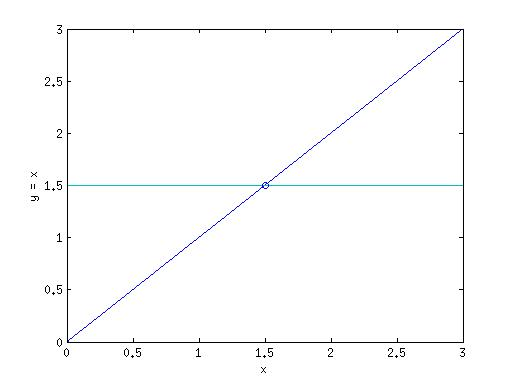
\includegraphics[scale=0.50]{fig/punto_medio.jpg}\end{center}
\caption{Integrale della funzione $f(x) = x$ nell'intervallo $(0,3)$ mediante
la formula del punto medio.}
\label{fig_puntomedio}\end{figure}

La formula del punto medio integra \emph{perfettamente} i polinomi di primo
grado (e inferiori), questo si può osservare chiaramente nell figura 
\ref{fig_puntomedio}.


\subsection{Errore di integrazione numerica.}
Analogamente a quanto fatto per le formule di Newton-Cotes chiuse, analizziamo
il resto dell'integrazione per stimarne l'errore.

\begin{teo}
Sia $n \in \nn$ dispari e $f \in \cc^{n+1}([a,b])$, allora esiste $\xi \in
(a,b)$ tale che:
\[
R_n(f) = K_n \cdot \frac{f^{n+1}(\xi)}{(n+1)!} \cdot h^{n+2}, \quad 
h = \frac{b-a}{n+2};
\]
\[
K_n = \int_{-1}^{n+1}\mathcal{T}_ndt, \quad \mathcal{T}_n = \prod_{i=0}^n(t-i).
\]
\end{teo}
\begin{teo}
Sia $n \in \nn$ pari e $f \in \cc^{n+2}([a,b])$, allora esiste $\xi \in
(a,b)$ tale che:
\[
R_n(f) = K_n \cdot \frac{f^{n+2}(\xi)}{(n+2)!} \cdot h^{n+3}, \quad 
h = \frac{b-a}{n+2};
\]
\[
K_n = \int_{-1}^{n+1}\mathcal{T}_ndt, \quad \mathcal{T}_n = \prod_{i=0}^n(t-i).
\]
\end{teo}
\begin{cor}
Le formule di Newton-Cotes aperte con $n$ dispari hanno grado di precisione
$n$, quelle con $n$ pari hanno grado di precisione $n+1$.
\end{cor}

\begin{osse}
In particolare la formula del punto medio integra \emph{esattamente} tutti i
polinomi di grado $\leq 1$.
\end{osse}

\begin{prop}
Sia $f \in \cc^{2}([a,b])$, ovvero $n = 0$, allora l'errore risulta:
\[
R_0(f) = \frac{1}{3}f''(\xi)h^3, \quad h = \frac{b-a}{2}.
\]
\end{prop}
\begin{dimo}
Poniamo $f$ nella generica ``forma di secondo grado'' $f(x) = (x-c)^2$, il
punto medio $x_0=\frac{a+b}{2}$ e $p$ il polinomio al più di primo
grado che interpola $f$ nel punto $x_0$. Sia ora la derivata prima
calcolata in $x_0$ uguale a $c$, ovvero $f'\left(x_0\right) = c$.

\[\begin{array}{lclr}
R_0(f) &=& \displaystyle \int_a^bf(x)dx - h\cdot \alpha_0 
\cdot f\left(x_0\right) & \textrm{per def.} \\
&=& \displaystyle\int_a^bf(x)dx - \underbrace{h\cdot \alpha_0\cdot
 p\left(x_0\right)}_{* = \int_a^bp(x)dx}& \textrm{def. di interpolazione}\\
&=& \displaystyle\int_a^b\left[f(x)-p(x)\right]dx & *\\
&=& \displaystyle\int_a^b\frac{(x-c)^2f''(\xi)}{2!}dx 
& \textrm{def. di errore di interp.}\\
&=& \displaystyle\frac{f''(\xi)}{2}\int_a^b(x-c)^2dx. & \textrm{teo. media gen.}
\end{array}\]
Poniamo ora $x = a + (t+1)\cdot h$, abbiamo che:
\[\begin{array}{lcl}
R_0(f) &=& \displaystyle\frac{f''(\xi)}{2}\int_{-1}^1t^2h^2hdt \\
&=& \displaystyle\frac{f''(\xi)}{2}\int_{-1}^1t^2h^3dt\\
&=& \displaystyle\frac{f''(\xi)}{2}\cdot h^3 \int_{-1}^1t^2dt \\
&=& \displaystyle\frac{f''(\xi)}{2}\cdot h^3 \left[\frac{t^3}{3}\right]_{-1}^1\\
&=& \displaystyle\frac{1}{3}\cdot h^3 \cdot f''(\xi).
\end{array}
\]
\end{dimo}
